Per misurare il momento d'inerzia si è proceduti per due modi: metodo geometrico e metodo dinamico.

\subsubsection*{Metodo geometrico}

La geometria del disco non omogeneo è stata valutata prendendo misure delle dimensioni dei vari toroidi, numerati per semplicità da 1 a 4 a partire da quello più interno. In Fig. \ref{sezione} è possibile visualizzare la proiezione ortogonale della semisezione assiale del disco.
    \begin{figure}[h]
        \centering
        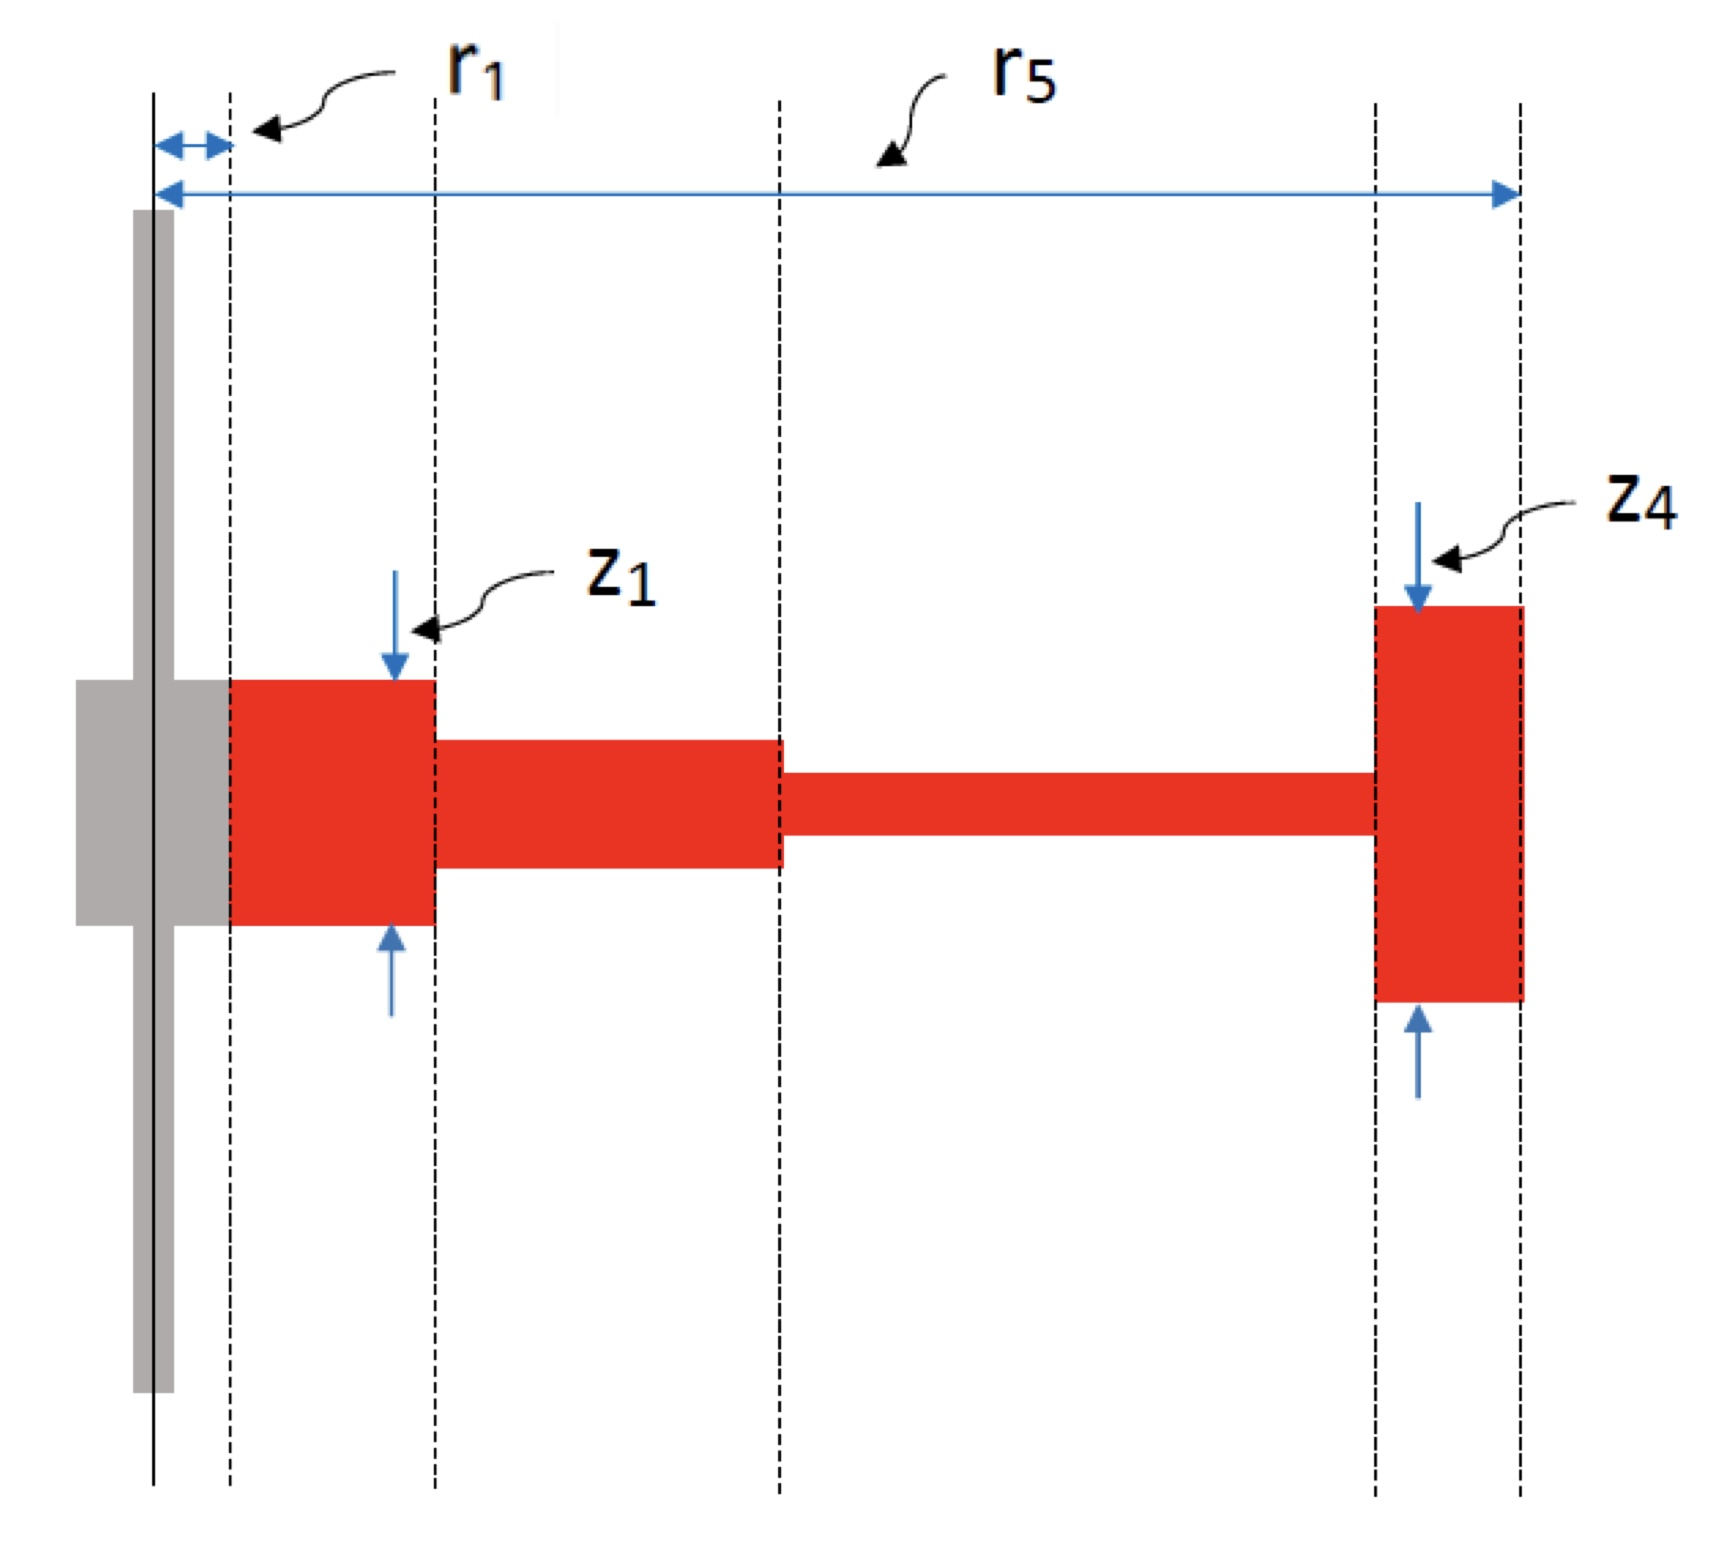
\includegraphics[width=0.6\textwidth]{image/Sezionedisco.jpeg}
        \caption[\small Visualizzazione della semisezione assiale del disco.]{\small Visualizzazione della semisezione assiale del disco. La parte grigia della sezione corrisponde al perno metallico, mentre le parti rosse indicano i toroidi. $r_1$ e $r_5$ sono rispettivamente il raggio interno del primo toroide e quello esterno della quarta, mentre $z_1$ e $z_4$ indicano rispettivamente lo spessore del primo toroide e della quarta.}
        \label{sezione}
    \end{figure}\\
Quindi si è andati a misurare i diametri dei toroidi e i vari spessori con il calibro digitale, mentre per la densità era già data \textit{a priori}.
Per misurare i diametri $d_i$ si sono fatte 3 misure per ogni grandezza, tranne per $d_1$, per il quale si sono fatte 5 misure, perché nell'utilizzo del calibro il luogo in corrispondenza del diametro più interno non aveva punti fissi d'appoggio.\\
Invece per i spessori $z_i$ la situazione è diversa: si può misurare direttamente solo lo spessore più esterno $z_4$, mentre per i restanti, considerando solo una faccia del disco, è stato possibile misurare le tre profondità presenti, numerate da 1 a 3 dall'interno verso l'esterno (Fig. \ref{profondità}). In questo caso sono state fatte quattro misure per ogni grandezza.
    \begin{figure}[htbp]
        \centering
        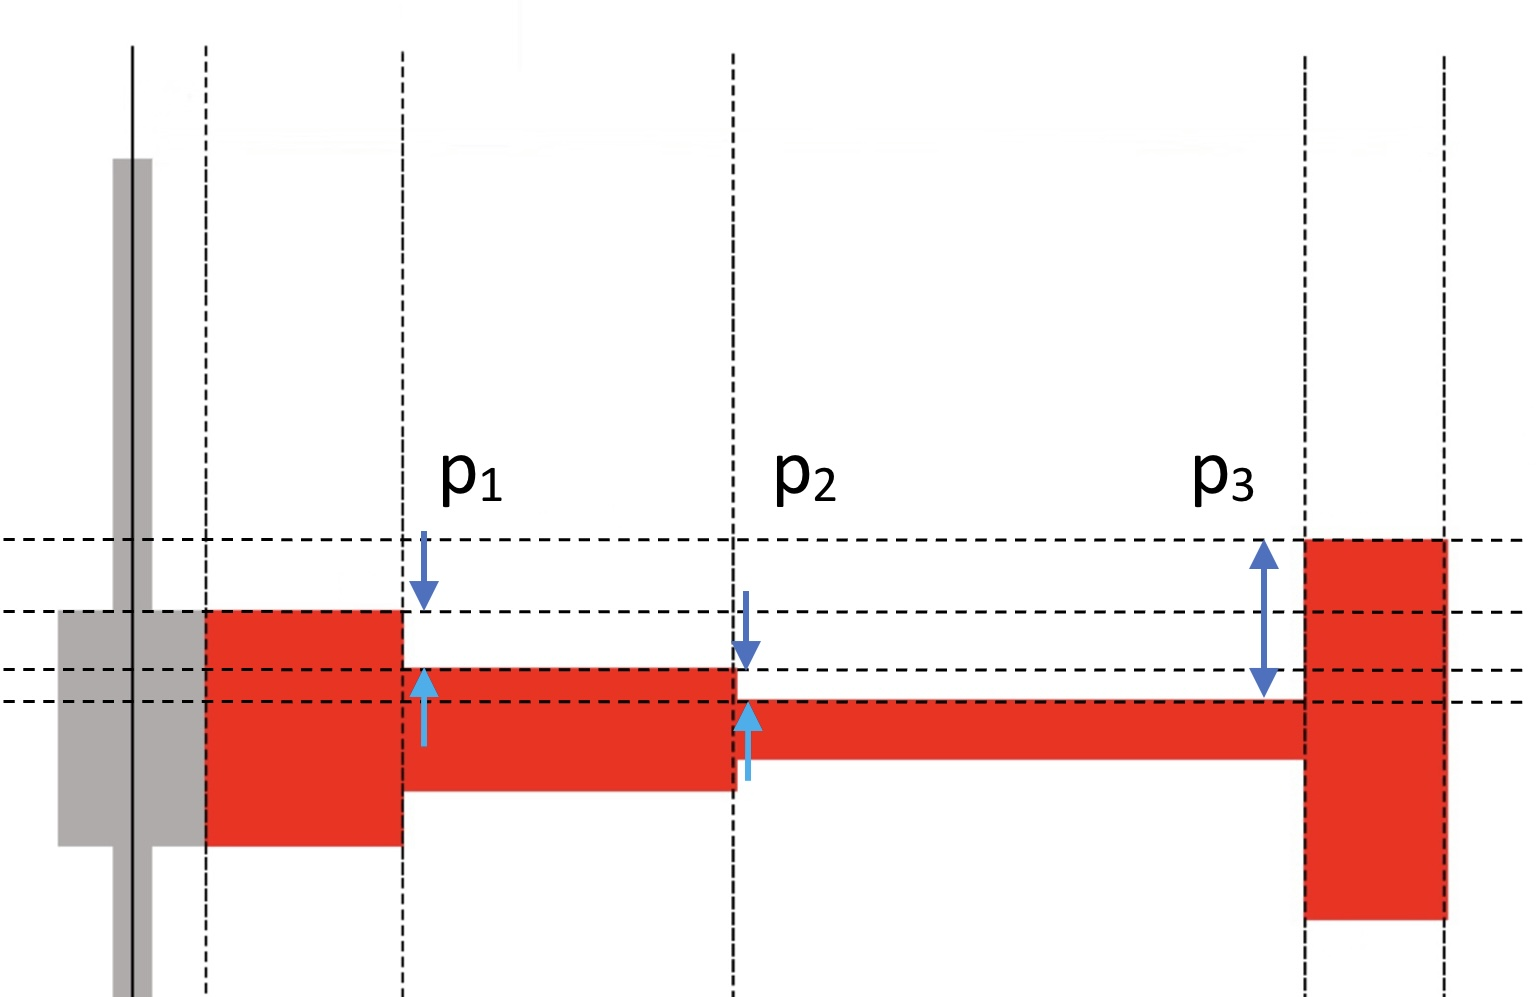
\includegraphics[width=0.75\textwidth]{image/Profondità.jpeg}
        \caption[\small Visualizzazione della semisezione assiale del disco - profondità]{\small Visualizzazione della semisezione assiale del disco. Vengono indicate in particolare le profondità da misurare con il calibro: $p_1$, $p_2$, $p_3$.}
        \label{profondità}
    \end{figure}\\
Per ogni toroide poi si è andati a calcolare il suo momento d'inerzia $I_i$ secondo la formula
$$\displaystyle I_i = \frac{\rho \pi}{32} \cdot z_i (d_{i+1}^4 - d_i^4) $$
con $\rho$ la densità del toroide, $z_i$ lo spessore del toroide $i$, $d_i$ il diametro interno del toroide e $d_{i+1}$ il diametro esterno.\\
Come abbiamo visto, il momento d'inerzia è additiva per oggetti rotanti sullo stesso asse, perciò il momento d'inerzia totale $I_G$ calcolato geometricamente equivale a
\begin{equation} \label{I_G}
    \displaystyle I_G = \sum_{i=1}^4  I_i = \frac{\rho \pi}{32} \cdot \sum_{i=1}^4 z_i (d_{i+1}^4 - d_i^4)
\end{equation}

\subsubsection*{Metodo dinamico}
Per il calcolo del momento d'inerzia ricorrendo per metodo dinamico si è utilizzato il pendolo di Maxwell, perché è necessario il \textbf{tempo di caduta} del disco $t_o$. Per far ciò si è andati ad utilizzare il cronometro digitale.\\
Chiamando per semplicità la posizione iniziale del disco “posizione di quiete", arrotolando il filo attorno il perno metallico, il disco si porta lentamente il alto, fino a raggiungere all'\textbf{altezza massima} $h_o$, misurata 3 volte rispetto alla posizione di quiete con il metro a nastro; lasciando cadere il disco questo assume un moto rototraslatorio uniformemente accelerato verso il basso, fino a raggiungere la posizione di quiete. Il cronometro viene fatto partire dall'instante in cui si lascia il disco e fatto fermare quando raggiunge la posizione di quiete.\\
Visto che la misura di $t_o$ è influenzato dal nostro tempo di reazione, allora si è andati a ripetere  40 volte lo stesso procedimento. Distribuendo le 40 misure in bin da 0.1 s, si è fatto la media per ottenere $t_o$.\\
Inoltre sono state effettuate misure del \textbf{diametro del perno metallico e dei fili}, rispettivamente $d_p$ e $d_f$, attraverso l'utilizzo del micrometro, effettuando 3 misure per ciascuna grandezza.
Per quanto riguarda invece la massa del disco $m$, il valore è stato fornito \textit{a priori}.\\

Ottenuti i parametri si può andare a calcolare il valore del momento d'inerzia del disco $I_D$ mediante metodo dinamico con la seguente formula:
\begin{equation} \label{I_D}
\displaystyle I_D = \frac{m(d_p + d_f)}{8h_o}(gt_o^2+2h_o)
\end{equation}
con $g$ l'accelerazione di gravità terrestre.